\documentclass[reprint, aps, prx, amsmath, amssymb, longbibliography, superscriptaddress]{revtex4-2}

%% don't need amsmath because it is loaded in \documentclass
%% \usepackage{amsmath,amssymb}
\usepackage{graphicx}
\usepackage{epsfig}
\usepackage{mathrsfs,esint}
\usepackage{physics}
\usepackage{relsize}
%% \usepackage{float} %% revtex4-2 has a conflict with float
\usepackage{dsfont}
\usepackage{comment}
\usepackage{svg}

%% packages for combining several images into a single figure
%%\usepackage{caption}
%%\usepackage{subcaption}
\usepackage[caption=false]{subfig}

%% Hyperref loaded the last because some packages may redefine \label
\usepackage[bookmarks=true,
   colorlinks=true,
   linkcolor=blue,
   urlcolor=blue,
   citecolor=blue,
   bookmarks=true,
   hyperindex=true
]{hyperref}
%\usepackage{natbib}

\definecolor{mediumtealblue}{rgb}{0.0, 0.33, 0.71}
\newcommand{\jk}[1]{{\color{mediumtealblue}#1}}
\newcommand{\al}[1]{{\color{purple}#1}}
\newcommand{\dl}[1]{{\color{red}#1}}


\DeclareMathOperator{\Zn}{\mathbb{Z}_n}
\DeclareMathOperator{\Zthree}{\mathbb{Z}_3}
\DeclareMathOperator{\Ztwo}{\mathbb{Z}_2}
\DeclareMathOperator{\Id}{Id}
\DeclareMathOperator{\diag}{diag}
\DeclareMathOperator{\sgn}{sign}


\begin{document}
\subsection{Superconducting circuit implementation}
\label{superconducting-implementation}


The obvious choice for boson modes is an LC circuit. For the qubit ($\sigma_i$)  we consider superconducting charge qubits \cite{bouchiat_quantum_1998,nakamura_coherent_1999,lehnert_measurement_2003,makhlin_quantumstate_2001}, because we want the qubit eigenstate to be a charge state. More extensive discussion on the charge qubits we use is provided in App. \ref{charge-qubit}. Here, we only want to comment that the qubit eigenstates are $|0\rangle, |1\rangle$ defined by $\hat n |0\rangle = 0, \, \hat n |1\rangle = |1\rangle$, where $\hat n$ is the capacitor charge operator. Below, to denote a linear span of these states we use $\mathcal{V}_k = \operatorname{Span}\{|0\rangle_k, \, |1\rangle_k\}$ where $k$ is the number of the qubit.

Fig.~\ref{fig:superconducting-Rabi} shows a superconducting realization of the three‑site qubit–boson ring. Each horizontal branch of the circuit (Fig.~\ref{fig:superconducting-Rabi}) correspond to site $i = 0,1,2$ of the qubit-boson ring. The $i$th boson and qubit are implemented by the LC circuit and SC qubit on the $i$th branch respectively. The JJs on the on the vertical segments of the circuit on the right of Fig.~\ref{fig:superconducting-Rabi} are responsible for the interaction term in $H_{QB}$~\eqref{physical-hamiltonian} \cite{siewert_aspects_2000,rasmussen_controllable_2019,shafranjuk_twoqubit_2006,allman_tunable_2014,hu_controllable_2007}. On Fig.~\ref{fig:superconducting-Rabi} is, the characteristic parameters of every circuit element are also shown: LC circuit's conductor and inductor have capacitance $C_{\text{B}}$ and inductance $L_{\text{B}}$ respectively. The qubit's JJ and capacitance have critical current $I_{\text{Q}}$ and capacitance $C_{\text{Q}}$ respectively. The coupling JJs on the right have critical current $I_{\text{R}}$. For clarity, we omit any elements that are necessary for an actual experimental implementation, e.g., read‑out resonators, flux‑bias lines, and filtering components.

\begin{figure}[t]
  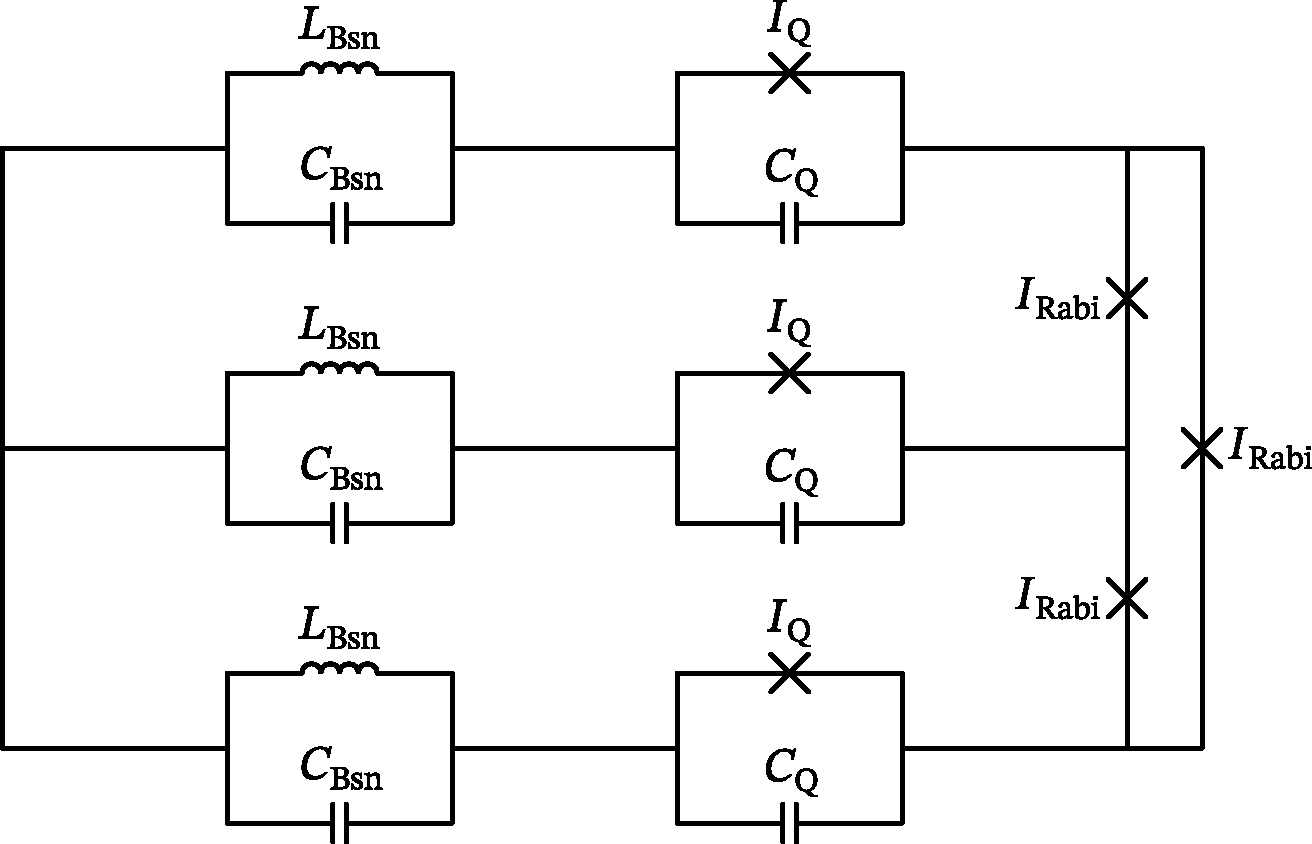
\includegraphics[width=\linewidth]{pics/SC_Rabi_circuit_svg-tex.pdf}
  \caption{Superconducting circuit implementation of the 2-mode $\Zthree$ Rabi model $\hat H_{\text{R}2}$. The LC circuits $(L_{\text{B}}, C_{\text{B}})$ host the boson modes; the charge qubits $(I_{\text{Q}}, C_{\text{Q}})$ correspond to the qubit degrees of freedom; Josephson junctions $I_{\text{Rabi}}$ are responsible for the interaction term in the qubit-boson ring. Altogether, the circuit is described by the Hamiltonian (\ref{physical-hamiltonian}).}
  \label{fig:superconducting-Rabi}
\end{figure}

Next, we describe why this circuit models the Hamiltonian~\eqref{physical-hamiltonian}. Without the coupling JJs, the LC circuits and qubits are independent from each other and are described by a non-interacting Hamiltonian:
\begin{equation}
  \hat H = \sum_{i = 0}^2 \hat H_{LC, i}(\phi_i, q_i) + \sum_{i = 0}^2 \hat H_{Q,i}(\varphi_i, n_i),
\end{equation}
where $ \phi_i, q_i$ are the magnetic flux and the capacitor charge of the $i$th LC circuit, while $\varphi_i, n_i$ are the JJsuperconducting phase and capacitor charge of the qubit. The LC circuit Hamiltonian is obviously $ H_{LC, i} = q_i^2/(2C) + \phi_i^2/(2L)$. Meanwhile, we leave the qubit Hamiltonian $\hat H_{Q,i} $ generic to allow different qubit types. However, we require the qubit to be a charge qubit and satisfy the following properties:
\begin{align}
   \hat H_{Q}\bigg|_{\mathcal{V}} = \begin{pmatrix} \bra{0_i}\hat H_Q\ket{0_i} & \bra{0_i} \hat H_Q \ket{1_i} \\ \bra{1_i} \hat H_Q \ket{0_i} & \bra{1_i} \hat H_Q \ket{1_i} \end{pmatrix} = \epsilon \sigma_z,
\end{align}
where the qubit states $\ket{0_i},\ket{1_i}$ are the charge operator eigenstates $ \hat q_i \ket{0_i} = Q \ket{1_i}, \, \hat q_{i} \ket{1}_i = (Q+1)\ket{1}_i$ with $ Q \in \mathbb{Z}$. $\mathcal{V}_i = \operatorname{Span}\{\ket{0_i},\, \ket{1_i}\}$ is a qubit Hilbert space, i.e, a computational subspace of the full Hilbert space of the qubit system $ \hat H_{Q,i}$. Due to this property, the operator $ e^{i\varphi_i} $ acts on the qubit subspace $\mathcal{V}_i$ as a raising operator:
\begin{equation}
  \begin{aligned}
    &e^{i\hat\varphi_i}\bigg|_{\mathcal{V}_i} = \begin{pmatrix} \bra{0_i} e^{i\hat\varphi_i} \ket{0_i} & \bra{0_i} e^{i\hat\varphi_i} \ket{1_i} \\ \bra{1_i} e^{i\hat\varphi_i} \ket{0_i} & \bra{1_i} e^{i\hat\varphi_i} \ket{1_i} \end{pmatrix} = \sigma^+,
  \end{aligned}
\end{equation}
because $[e^{i\phi}, n] = e^{i\phi}$.

If we now connect the $i$th and $(i+1)$th circuit branches with a JJ, it creates a cycle in the circuit. As a result, the fluxes and the superconducting phases have to satisfy a requirement:
\begin{equation}
  \hat \phi_i + \hat\varphi_i + \hat\varphi_R - \hat\varphi_{i+1} - \hat\phi_{i+1} = 2\pi N, \, \text{where}\ N \in \mathbb{Z}.
\end{equation}
In other words, the superconducting phase $\phi_R$ of the coupling JJ is not an independent degree of freedom. Therefore, for the corresponding term in the Hamiltonian we obtain:
\begin{equation}
    \hat V_{\text{SC QB},j} = I_{\text{R}} \cos(\hat \phi_R) =  I_{\text{R}}\cos(\hat \phi_j + \hat \varphi_j - \hat \phi_{j+1} - \hat \varphi_{j+1}).
\end{equation}


As we are only interested in qubit states $|0\rangle_k,\, |1\rangle_k$, we restrict the JJ term $\hat V_{\text{SC QB},j}$ to the qubit Hilbert subspace $\mathcal{V}_j\otimes \mathcal{V}_{j+1}$:
\begin{equation}
\begin{aligned}
    &\hat V_{\text{SC QB},j} \bigg |_{\mathcal{V}_j\otimes \mathcal{V}_{j+1}} = \\
    &=\frac{I_{\text{Rabi}}}{2}\left(e^{i(\hat\varphi_j - \hat\varphi_{j+1})} e^{i(\hat\phi_j - \hat\phi_{j+1})} + h.c. \right) \bigg|_{\mathcal{V}_j\otimes \mathcal{V}_{j+1}} \\
    &=\frac{I_{\text{Rabi}}}{2}\left(e^{i(\hat\varphi_j - \hat\varphi_{j+1})} \sigma_j^- \sigma_{j+1}^+ + h.c. \right).
\end{aligned}
\end{equation}
Here we used the fact that $e^{\pm i\hat\phi}$ acts as a raising/lowering operator for the charge qubit: $e^{i\hat\phi}|_{\mathcal{V}} = \sigma^+$. Hence the need for charge qubits rather than flux or phase qubits.

The Josephson junction coupling between two pairs of an LC circuits and a charge qubits gives us precisely the interaction term we wanted. As a result, we conclude that the system depicted in Fig. \ref{fig:superconducting-Rabi} is described by the Hamiltonian (\ref{physical-hamiltonian}).  The qubit-boson ring couplings can be expressed by the circuit parameters:
\begin{equation}
\begin{aligned}
    &\epsilon = \frac{\delta}{2 C_Q},\,
    \Omega_{QB} = \left(\sqrt{L_{\text{B}}C_{\text{B}}}\right)^{-1/2}, \\
    &m_{QB} = C_{\text{B}}, \, g = \frac{I_{\text{Rabi}}}{2}.
\end{aligned}
\end{equation}
For details of the $\epsilon$ computation, see App. \ref{charge-qubit}. Finally, applying Sec. $\ref{physical-implementation}$ argument we deduce that the circuit is described by the $\Zthree$ Rabi model.


\end{document}